\chapter{Application Design}
\textit{In this chapter we will present the design for our android application and short describe which feature the application will contain, what the d and why we have choses these features to the android application.}\\
\label{appdes}
\\
Based on the original design for the Digi-Pecs application, modified by the information gathered in the previous chapters, we have come up with the general idea for how we want the design for PARROT to be.\newline
First of all, we want the application to be safe, simple to use, and easy to remember.\newline
By \textit{safe}, we mean that the users of the system should only have access to their own area. For instance, a child user should not (commonly) have access to the options and administration parts of the application, while guardians should not have access to the profiles of other guardians, or children not under their supervision.\newline
For the system to be \textit{simple to use} and \textit{easy to remember}, we want the application to have a relatively simple user interface. Especially because the application is meant to be used by children with autism. Furthermore, the reason for making this application is to make the daily use of pictograms easier. This goes for the guardians as well. If they can't use the system, the children will not be able to learn how to use it.\newline
Based on the fact that we are making a digital version of the daily use of pictograms, we want to expand the concept of pictogram, meaning that not only will the pictogram contain a picture and a string of text, it will now also contain sound in the form of a pronunciation of the word, as well as a sound effect.
It is not our thought that the system has to be intuitive, but it is our opinion that if the user is provided by a short demonstration or manual, they will master the concepts of the application in no time.\newline
\\
Designing the user interface has been an iterative process, such is the method of SCRUM. We started by having a look at the design from the report of the previous year (we were unable to see the actual design) and compared it to the tools shown to us by Tove S\o{}by.%skal der refereres ved navn?
We decided that we wanted our design to look and feel like the real thing, so we drew up a quick sketch of how the system would look in our opinion.\newline
\begin{figure}[htbp]
	\centering
		%\includegraphics{}
	\caption{Sketch of the speech board tab}
	\label{sketchspeech}
\end{figure}
%indsaet billede
As seen in the picture, we wanted a speech board to show the current available pictograms, a sentence board to put the pictograms on to create a sentences, and a number of tabs representing different categories of pictograms. We also put a play-button on the design, so that the user could press it to play out the sentence.\newline
The reason for this choice was based on the idea of having the system be as close to the existing tools as possible. The guardians already have speechboards and sentence boards, and they have lots of folders containing pictograms organized into different categories. This is why we went for the tab style for the categories, as that would make it look more like a folder.\newline
As we began implementing the system, we realized that we had to make several changes. First of all, the size of the initial sentenceboard was too small, it would have to be bigger in order to make the pictograms easily visible. Also, we had to change the design from tabs to buttons, as we discovered that Android does not natively support vertical tabs. We also removed the play-button, mainly because our contact said that she would rather have the ability to play each pictogram one at a time, than only the ability to play the entire sentence. Also, the button took up a lot of the already limited space on the interface.\newline
\\
After designing of the speech board, we continued on to the parts of the application that is restricted to the guardians. We had to make the design so that the options and the administrations where easy to access for the guardian when they need to make changes for the specific child that is using the application. 
\\
We tried to see what the application from last year did but this was not possible so we began to search for other ways to do so. We came up with idea for a tab for the speech board, a tab for options and a tab for the administrations for categories.\\

The design for the administration for categories see figure \ref{fig:admincate}. First we have a spinner that contains the available profiles. Below this we have a list of  categories for the selected profile. Below that we have a trash bin to dispose of unwanted objects. In the upper right corner we have the selected category information shown, in this box we can change all information regarding the selected category. Below that we have all the pictogram that is found in the selected category.       

\begin{figure}[htbp]
	\centering
		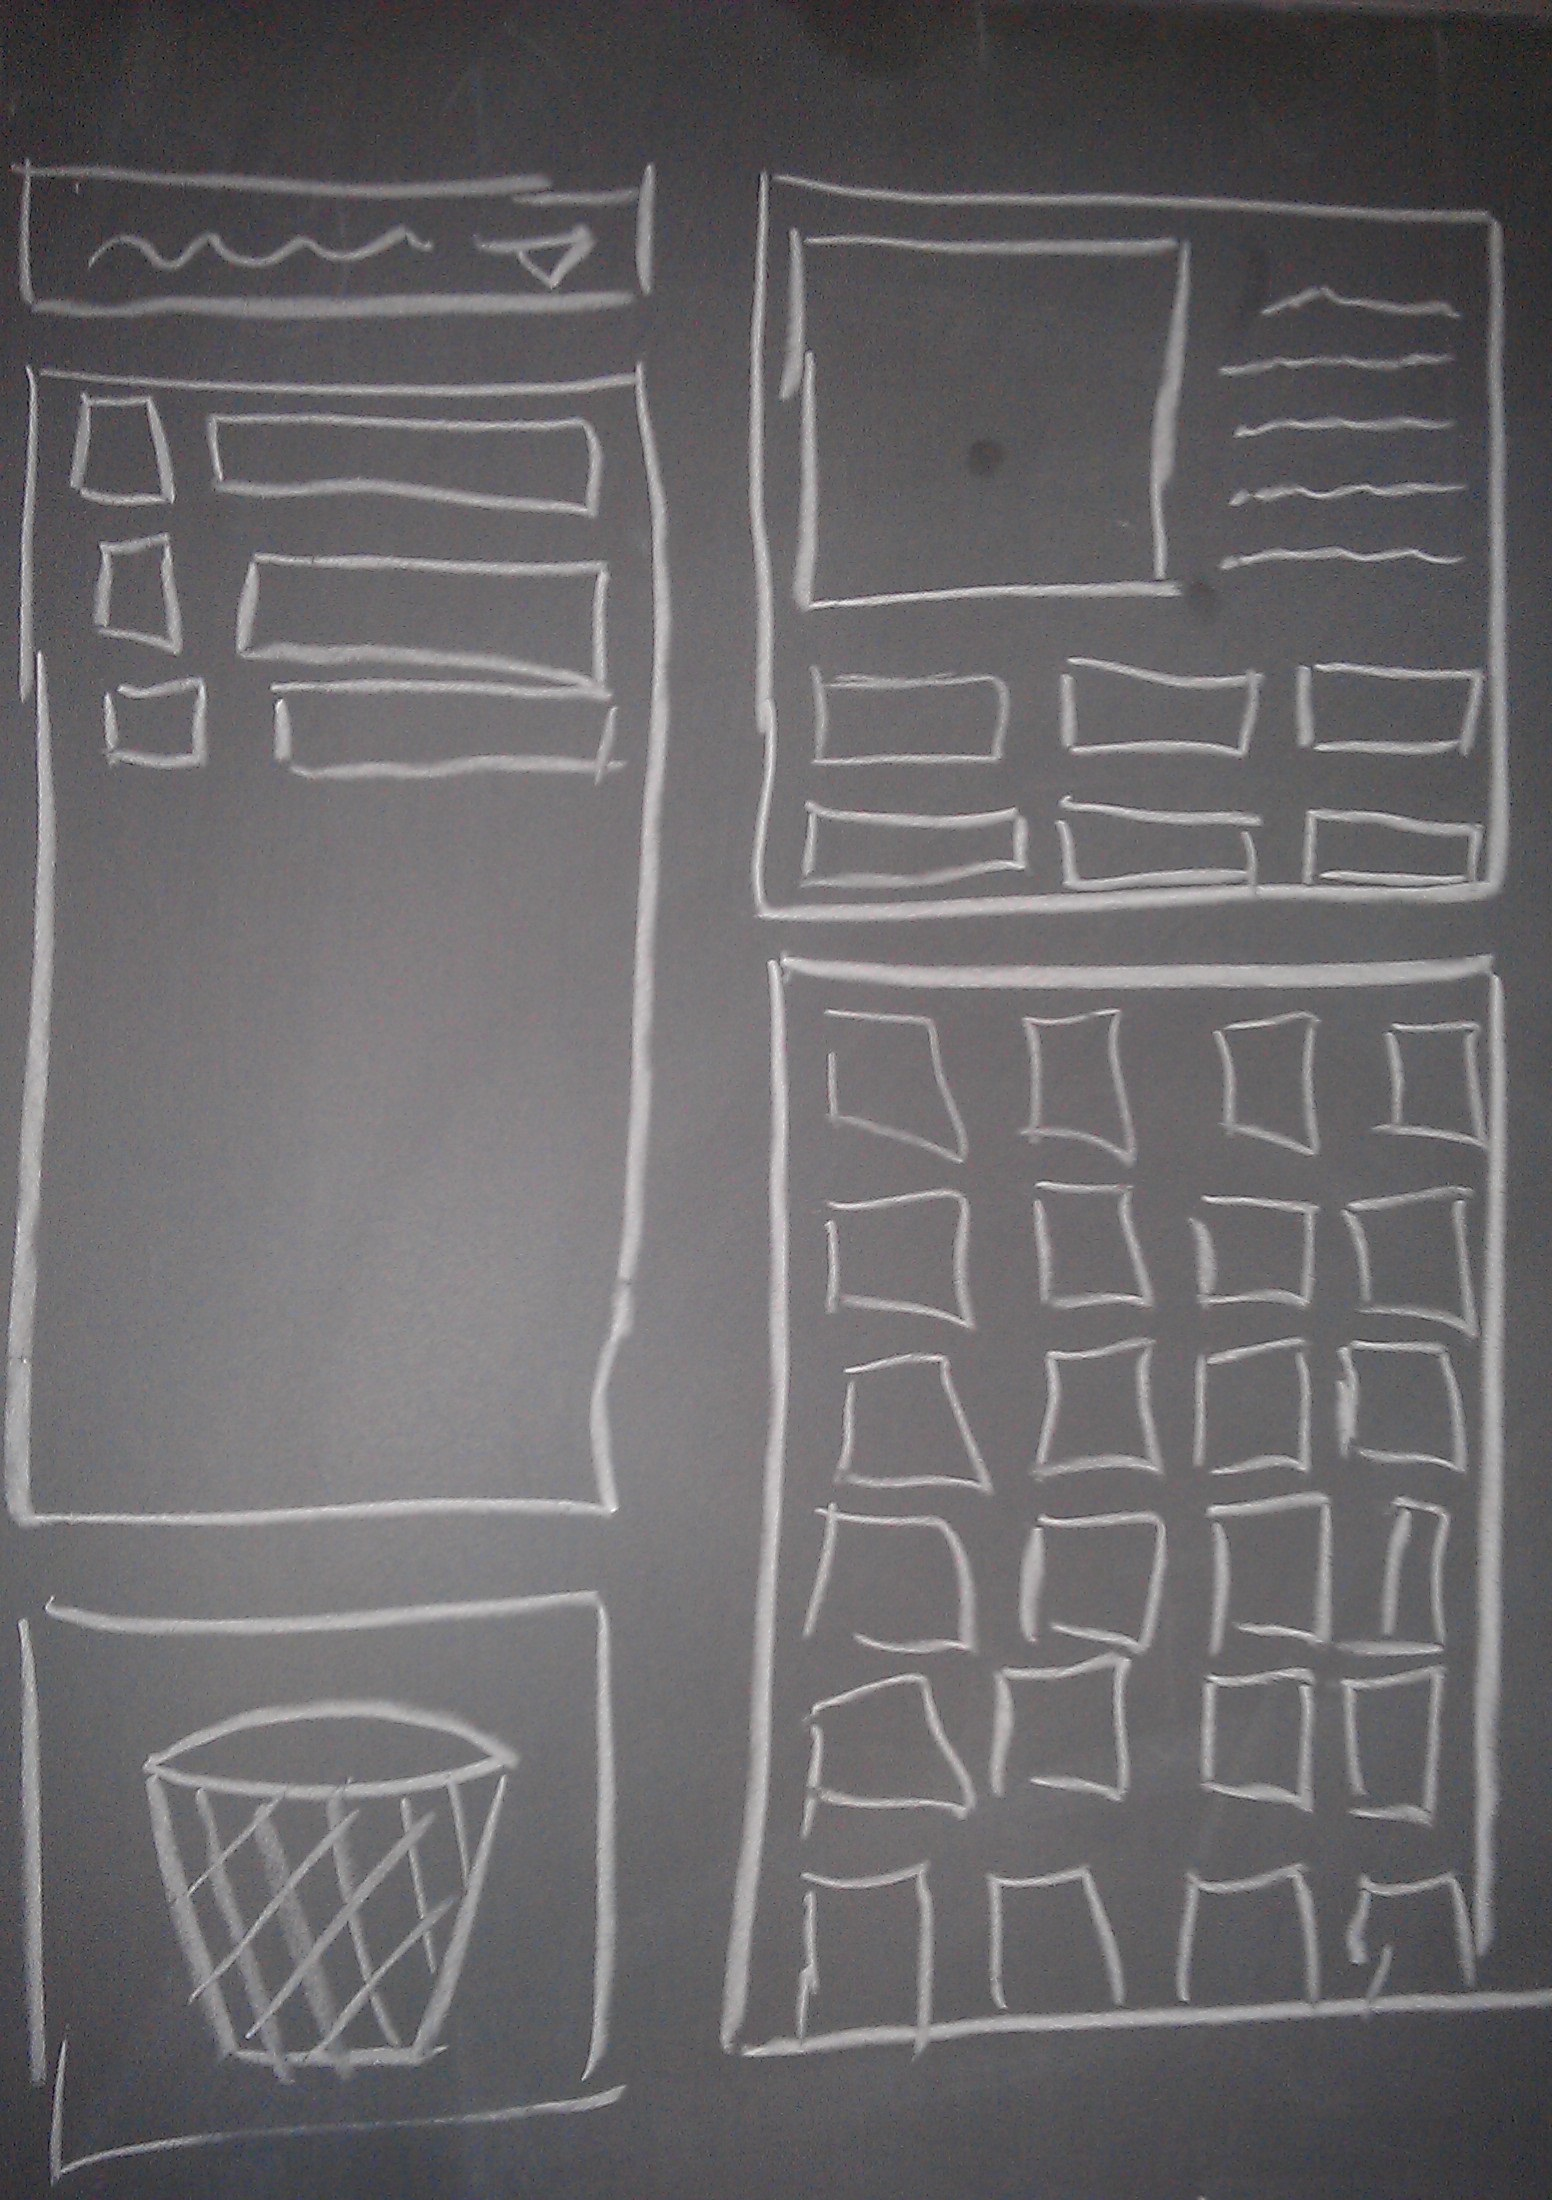
\includegraphics[scale=0.10]{input/images/admincate.jpg}
	\caption{Sketch of admin for categories}
	\label{fig:admincate}
\end{figure}

Now we had been through the design for the application, we also have a lot of features for the application: 

\begin{itemize}
	\item \textbf{Drag and Drop:} This feature allows the user to choose a pictogram and drag, it to it's destination and drop the pictogram.  We choose this feature for the application because we want the application to simulate how the pictograms are used normally, meaning that the user has some pictograms and can ``pick up'' a pictogram and put it on the sentence board.  
	\item \textbf{Sound:} This feature enables us to play the audio track that is a part of the pictogram. The feature was chosen because we need a way so the user of the application can play the sound of the pictogram. 
	\item \textbf{Action Bar:} This feature allows us to use tabs in the application. We are using this feature so that the options and administration of categories would be easy to access for the guardian. 
	\item \textbf{Color Picker:} This feature gives the user a color scheme so that the user can choose which color the speech board tab should have and the color picker is also used when the guardian chooses color of the categories. We use this feature because one of main points in our application is that we can adjust the application to needs of each child. 
	\item \textbf{Showing Pictogram:} This feature takes the pitograms that is a part of the users profile and put it into the pictogram grid in the speech board tab. This feature is important for it is the part that gives us our pictograms. 
	\item \textbf{Sentence Board:} This part of the speech board is where the user can drag pictograms down onto and arranges the chosen pictograms so that the user can make a sentence. It is also where the user can play the audio track in the pictogram. This feature is essential for our application since that is it all this application is about. 
	\item \textbf{Data Management:} This is the part where we access the database to get the profiles and pictograms used by the application.
\end{itemize}

So with these designs see figure \ref{sketchspeech} and see figure \ref{fig:admincate} we contacted Tove to get some feedback for the designs and she gave a positive feedback so we put our design in to production.\\  
\\
\textit{The design for our android application has now been presented with sketches for the different tab of the application furthermore we have presented the  features for our application and described how imported they are for the end product.} 